\providecommand{\econtexRoot}{}
\renewcommand{\econtexRoot}{..}
\providecommand{\econtexPaths}{}\renewcommand{\econtexPaths}{\econtexRoot/Resources/econtexPaths}
% The \commands below are required to allow sharing of the same base code via Github between TeXLive on a local machine and Overleaf (which is a proxy for "a standard distribution of LaTeX").  This is an ugly solution to the requirement that custom LaTeX packages be accessible, and that Overleaf prohibits symbolic links
\providecommand{\econtex}{\econtexRoot/Resources/texmf-local/tex/latex/econtex}
\providecommand{\econtexSetup}{\econtexRoot/Resources/texmf-local/tex/latex/econtexSetup}
\providecommand{\econtexShortcuts}{\econtexRoot/Resources/texmf-local/tex/latex/econtexShortcuts}
\providecommand{\econtexBibMake}{\econtexRoot/Resources/texmf-local/tex/latex/econtexBibMake}
\providecommand{\econtexBibStyle}{\econtexRoot/Resources/texmf-local/bibtex/bst/econtex}
\providecommand{\econtexBib}{\econtexRoot/Resources/texmf-local/bibtex/bib/economics}
\providecommand{\notes}{\econtexRoot/Resources/texmf-local/tex/latex/handout}
\providecommand{\handoutSetup}{\econtexRoot/Resources/texmf-local/tex/latex/handoutSetup}
\providecommand{\handoutShortcuts}{\econtexRoot/Resources/texmf-local/tex/latex/handoutShortcuts}
\providecommand{\handoutBibMake}{\econtexRoot/Resources/texmf-local/tex/latex/handoutBibMake}
\providecommand{\handoutBibStyle}{\econtexRoot/Resources/texmf-local/bibtex/bst/handout}

\providecommand{\FigDir}{\econtexRoot/Figures}
\providecommand{\CodeDir}{\econtexRoot/Code}
\providecommand{\DataDir}{\econtexRoot/Data}
\providecommand{\SlideDir}{\econtexRoot/Slides}
\providecommand{\TableDir}{\econtexRoot/Tables}
\providecommand{\ApndxDir}{\econtexRoot/Appendices}

\providecommand{\ResourcesDir}{\econtexRoot/Resources}
\providecommand{\rootFromOut}{..} % Path back to root directory from output-directory
\providecommand{\LaTeXGenerated}{\econtexRoot/LaTeX} % Put generated files in subdirectory
\providecommand{\econtexPaths}{\econtexRoot/Resources/econtexPaths}
\providecommand{\LaTeXInputs}{\econtexRoot/Resources/LaTeXInputs}
\providecommand{\LtxDir}{LaTeX/}
\providecommand{\EqDir}{Equations} % Put generated files in subdirectory
\documentclass[pdflatex]{beamer}
\providecommand{\texname}{ProjectKWK-Slides}% Indicate the keyname for the bibtex entry corresponding to this document
\providecommand{\texnameMaster}{ProjectKWK}% Indicate the keyname for the bibtex entry corresponding to this document
\newif\ifdvi\dvifalse

%\usepackage{optional}
\usepackage{ifthen}%\usepackage{\econtexRoot/ProjectKWK}

% Can't read in ProjectKWK.sty because some packages conflict with Beamer
% So need to redefine everything here

\usepackage{\econtexShortcuts}
\usepackage{natbib,amsmath,amssymb,rotating,subfigure}
\usepackage{verbatim,moreverb,graphicx}
\usepackage{wasysym}
\usepackage{dcolumn}
\usepackage{cancel}
\usepackage{booktabs}

%\providecommand{\LtxDir\EqDir}{\econtexRoot/Equations}
\providecommand{\FigsRaw}{\econtexRoot/Code/Python/Figures}
\providecommand{\CodeDir}{\econtexRoot/Code}
\providecommand{\CalibrationDir}{\econtexRoot/Calibration}
\providecommand{\TableDir}{\econtexRoot/Tables}
\providecommand{\ApndxDir}{\econtexRoot/Appendices}
\providecommand{\Ex}{\mathbb{E}}

%\usepackage{natbib}\newcommand*{\newblock}{}

\mode<presentation>
{
  \usetheme{Warsaw}
  % or ...
  \setbeamercovered{transparent}
}

%\beamerdefaultoverlayspecification{<+->}

%\setbeamertemplate{navigation symbols}{}  % Take away navigation symbols

\usetheme{Warsaw}

\setbeamersize{text margin left=3mm}
\setbeamersize{text margin right=3mm}


%_____________ Opening slide _______________________

\title[Close Elections]{Close Elections, Campaign Contributions, and Financial Deregulation}
\author[Koh]{Kyung Woong Koh}
\institute[JHU]{Johns Hopkins University}
\date[\today]{\today}

\begin{document}\bibliographystyle{\econtexBibStyle}

\begin{frame}[plain]
  \titlepage
\end{frame}


%_____________ 1st section  ____________
\section{Introduction}
\subsection{Motivation}


\begin{frame}
\frametitle{Introduction}

Are legislators in close elections more susceptible to special interests?
\begin{itemize}
	\item Answers within the context of financial deregulation
	\item Igan and Mishra (2014): Looks at legislators being susceptible to special interests of financial industry concerning deregulation of lending practices
	\item New contribution of this paper: Legislators in \textbf{close elections}
\end{itemize}
\end{frame}


\begin{frame}{Key Result}

\hypertarget{TestFig1}{}
\begin{figure}
\centerline{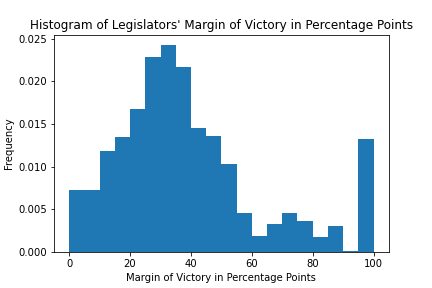
\includegraphics[width=6in]{\FigDir/TestFig1}}
\caption{Histogram of Legislators' Past Margin of Victory}
\label{fig:TestFig1}
\end{figure}

  
\end{frame}


\section{Mechanism}
\begin{frame}
\frametitle{Mechanism of Legislators' Vote Switching}

\begin{figure}[ht]
  \centerline{
    \includegraphics[width=0.8\textwidth]{\FigDir/KohFigure1_tikzmake}
  }
    \caption{Two Channels in which Legislators in Close Elections Switch their Votes Toward Financial Deregulation}\label{KohFigure1}
\end{figure}

\end{frame}


\section{Variables}

\begin{frame}
\frametitle{Dependent Variable}

\newsavebox{\DepVar}
\begin{table}
\centering
\caption{Definition of the Main Dependent Variable, Vote Switch towards Deregulation}\label{table:DepVar}
\sbox{\DepVar}{
\begin{tabular}{p{0.25\linewidth} | p{0.25\linewidth} | p{0.25\linewidth}} \hline
\textbf{Value of $S_iBR$}  & Voted for deregulation in Bill $B,R$ & Voted against deregulation in Bill $B,R$ \\ \hline
Voted for deregulation in Bill $B,R-1$ & 0 & 0 \\ \hline
Voted for deregulation in Bill $B,R-1$ & 1 & 0 \\ \hline
\end{tabular}
}
\usebox{\DepVar}
\end{table}

\end{frame}



\section{Regression Strategy}

\begin{frame}
\frametitle{Regression A-1}

Regression A1: Regression with only close election and relevant interaction terms
\begin{align}
    S_{iBR} &= \beta_{1} L_{BR} + \beta_{2} X_{iBR}^{P} + \beta_{3} (L_{BR} \times X_{iBR}^{P} ) \nonumber \\
    &+ \alpha F_{BR} + \gamma T_{BR}+ s_{i} \times t_{c}+ v_{B} \times t_{c}+\mu_{R} \times t_{c}+\varepsilon_{iBR}
\end{align}


\end{frame}


\begin{frame}
\frametitle{Results - Igan and Mishra (2014) Original Specification, OLS}

\begin{center}
\begin{tabular}{lclc}
\toprule
\textbf{Dep. Variable:}           &      sw\_p       & \textbf{  R-squared:         } &     0.039   \\
\textbf{Model:}                   &       OLS        & \textbf{  Adj. R-squared:    } &     0.038   \\
\textbf{Method:}                  &  Least Squares   & \textbf{  F-statistic:       } &     34.19   \\
\textbf{Date:}                    & Tue, 30 Nov 2021 & \textbf{  Prob (F-statistic):} &  1.19e-21   \\
\textbf{Time:}                    &     14:37:09     & \textbf{  Log-Likelihood:    } &   -1632.7   \\
\textbf{No. Observations:}        &        2517      & \textbf{  AIC:               } &     3273.   \\
\textbf{Df Residuals:}            &        2513      & \textbf{  BIC:               } &     3297.   \\
\textbf{Df Model:}                &           3      & \textbf{                     } &             \\
\bottomrule
\end{tabular}
\begin{tabular}{lcccccc}
                                  & \textbf{coef} & \textbf{std err} & \textbf{t} & \textbf{P$> |$t$|$} & \textbf{[0.025} & \textbf{0.975]}  \\
\midrule
\textbf{Intercept}                &       0.2290  &        0.115     &     1.995  &         0.046        &        0.004    &        0.454     \\
\textbf{log\_contributions\_FIRE} &       0.0033  &        0.010     &     0.350  &         0.726        &       -0.015    &        0.022     \\
\textbf{bill\_complexity}         &       0.0204  &        0.008     &     2.670  &         0.008        &        0.005    &        0.035     \\
\textbf{tight}                    &      -0.3406  &        0.038     &    -9.066  &         0.000        &       -0.414    &       -0.267     \\
\bottomrule
\end{tabular}
\begin{tabular}{lclc}
\textbf{Omnibus:}       & 14413.723 & \textbf{  Durbin-Watson:     } &    1.885  \\
\textbf{Prob(Omnibus):} &    0.000  & \textbf{  Jarque-Bera (JB):  } &  404.919  \\
\textbf{Skew:}          &    0.603  & \textbf{  Prob(JB):          } & 1.18e-88  \\
\textbf{Kurtosis:}      &    1.449  & \textbf{  Cond. No.          } &     157.  \\
\bottomrule
\end{tabular}
%\caption{OLS Regression Results}
\end{center}

Notes: \newline
 [1] Standard Errors assume that the covariance matrix of the errors is correctly specified.

\end{frame}


\begin{frame}
\frametitle{Results - Regression A2 (Election Closeness)}

\begin{center}
\begin{tabular}{lclc}
\toprule
\textbf{Dep. Variable:}           &      sw\_p       & \textbf{  R-squared:         } &     0.043   \\
\textbf{Model:}                   &       OLS        & \textbf{  Adj. R-squared:    } &     0.041   \\
\textbf{Method:}                  &  Least Squares   & \textbf{  F-statistic:       } &     22.51   \\
\textbf{Date:}                    & Tue, 30 Nov 2021 & \textbf{  Prob (F-statistic):} &  3.82e-22   \\
\textbf{Time:}                    &     14:37:09     & \textbf{  Log-Likelihood:    } &   -1627.9   \\
\textbf{No. Observations:}        &        2517      & \textbf{  AIC:               } &     3268.   \\
\textbf{Df Residuals:}            &        2511      & \textbf{  BIC:               } &     3303.   \\
\textbf{Df Model:}                &           5      & \textbf{                     } &             \\
\bottomrule
\end{tabular}
\begin{tabular}{lcccccc}
                                  & \textbf{coef} & \textbf{std err} & \textbf{t} & \textbf{P$> |$t$|$} & \textbf{[0.025} & \textbf{0.975]}  \\
\midrule
\textbf{Intercept}                &      -0.2967  &        0.224     &    -1.327  &         0.185        &       -0.735    &        0.142     \\
\textbf{log\_contributions\_FIRE} &       0.0488  &        0.019     &     2.632  &         0.009        &        0.012    &        0.085     \\
\textbf{mov\_past}                &       0.0135  &        0.005     &     2.946  &         0.003        &        0.005    &        0.022     \\
\textbf{mov\_contr\_int}          &      -0.0012  &        0.000     &    -3.023  &         0.003        &       -0.002    &       -0.000     \\
\textbf{bill\_complexity}         &       0.0203  &        0.008     &     2.666  &         0.008        &        0.005    &        0.035     \\
\textbf{tight}                    &      -0.3422  &        0.038     &    -9.117  &         0.000        &       -0.416    &       -0.269     \\
\bottomrule
\end{tabular}
\begin{tabular}{lclc}
\textbf{Omnibus:}       & 14833.066 & \textbf{  Durbin-Watson:     } &    1.886  \\
\textbf{Prob(Omnibus):} &    0.000  & \textbf{  Jarque-Bera (JB):  } &  399.670  \\
\textbf{Skew:}          &    0.601  & \textbf{  Prob(JB):          } & 1.63e-87  \\
\textbf{Kurtosis:}      &    1.463  & \textbf{  Cond. No.          } & 1.32e+04  \\
\bottomrule
\end{tabular}
%\caption{OLS Regression Results}
\end{center}

Notes: \newline
 [1] Standard Errors assume that the covariance matrix of the errors is correctly specified. \newline
 [2] The condition number is large, 1.32e+04. This might indicate that there are \newline
 strong multicollinearity or other numerical problems.

\end{frame}


\begin{frame}
\frametitle{Results - Regression C2 (Media Congruence)}

\begin{center}
\begin{tabular}{lclc}
\toprule
\textbf{Dep. Variable:}    &      sw\_p       & \textbf{  R-squared:         } &     0.046   \\
\textbf{Model:}            &       OLS        & \textbf{  Adj. R-squared:    } &     0.044   \\
\textbf{Method:}           &  Least Squares   & \textbf{  F-statistic:       } &     28.44   \\
\textbf{Date:}             & Tue, 30 Nov 2021 & \textbf{  Prob (F-statistic):} &  5.85e-18   \\
\textbf{Time:}             &     11:57:57     & \textbf{  Log-Likelihood:    } &   -1169.9   \\
\textbf{No. Observations:} &        1774      & \textbf{  AIC:               } &     2348.   \\
\textbf{Df Residuals:}     &        1770      & \textbf{  BIC:               } &     2370.   \\
\textbf{Df Model:}         &           3      & \textbf{                     } &             \\
\textbf{Covariance Type:}  &    nonrobust     & \textbf{                     } &             \\
\bottomrule
\end{tabular}
\begin{tabular}{lcccccc}
                          & \textbf{coef} & \textbf{std err} & \textbf{t} & \textbf{P$> |$t$|$} & \textbf{[0.025} & \textbf{0.975]}  \\
\midrule
\textbf{Intercept}        &       0.2349  &        0.046     &     5.056  &         0.000        &        0.144    &        0.326     \\
\textbf{congruence\_dc}   &      -0.0031  &        0.049     &    -0.063  &         0.950        &       -0.099    &        0.093     \\
\textbf{bill\_complexity} &       0.0332  &        0.009     &     3.646  &         0.000        &        0.015    &        0.051     \\
\textbf{tight}            &      -0.3527  &        0.046     &    -7.673  &         0.000        &       -0.443    &       -0.263     \\
\bottomrule
\end{tabular}
\begin{tabular}{lclc}
\textbf{Omnibus:}       & 8811.624 & \textbf{  Durbin-Watson:     } &    1.903  \\
\textbf{Prob(Omnibus):} &   0.000  & \textbf{  Jarque-Bera (JB):  } &  274.469  \\
\textbf{Skew:}          &   0.501  & \textbf{  Prob(JB):          } & 2.51e-60  \\
\textbf{Kurtosis:}      &   1.355  & \textbf{  Cond. No.          } &     25.0  \\
\bottomrule
\end{tabular}
%\caption{OLS Regression Results}
\end{center}

Notes: \newline
 [1] Standard Errors assume that the covariance matrix of the errors is correctly specified.

\end{frame}



\def\newblock{\hskip .11em plus .33em minus .07em}

\begin{frame}

\renewcommand{\bibsection}{\subsubsection*{\bibname }}

\tiny 

\bibliography{\texnameMaster,\econtexBib}

\end{frame}
\end{document}\endinput

% Local Variables:
% eval: (setq TeX-command-list  (remove '("Biber" "biber %s" TeX-run-Biber nil  (plain-tex-mode latex-mode doctex-mode ams-tex-mode texinfo-mode)  :help "Run Biber") TeX-command-list))
% eval: (setq TeX-command-list  (remove '("BibTeX" "%(bibtex) %s" TeX-run-BibTeX nil t                                                                              :help "Run BibTeX") TeX-command-list))
% eval: (setq TeX-command-list  (remove '("BibTeX" "%(bibtex) %s" TeX-run-BibTeX nil (plain-tex-mode latex-mode doctex-mode ams-tex-mode texinfo-mode context-mode) :help "Run BibTeX") TeX-command-list))
% eval: (setq TeX-command-list  (remove '("BibTeX" "%(bibtex) ../LaTeX/%s" TeX-run-BibTeX nil t :help "Run BibTeX")   TeX-command-list))
% eval: (add-to-list 'TeX-command-list	'("BibTeX" "%(bibtex) LaTeX/%s" TeX-run-BibTeX nil t :help "Run BibTeX") t)
% eval: (cond ((string-equal system-type "darwin") (progn (setq TeX-view-program-list '(("Skim" "/Applications/Skim.app/Contents/SharedSupport/displayline -b %n LaTeX/%o %b"))))))
% TeX-PDF-mode: t
% TeX-file-line-error: t
% TeX-debug-warnings: t
% LaTeX-command-style: (("" "%(PDF)%(latex) %(file-line-error) %(extraopts) -output-directory=LaTeX %S%(PDFout)"))
% TeX-source-correlate-mode: t
% TeX-source-correlate-start-server: 0
% TeX-parse-self: t
% End:
